\chapter{Outtakes from A grounding in the domain chapter}

The chapter continues with five practical aspects including app development and usage, information sources for developers, and choices for engaging with analytics. Developers need to address these as part of being effective in their work and providing apps of adequate quality. Mobile analytics can provide useful sources of information, including problems with the apps in use, and mobile analytics can complement and calibrate other sources of quality related information including software testing. 

\begin{comment}
    
%\textbf{How can we know about mobile analytics and the effects of using them?}

%\nth{16} Jul 2021:~\akb{This subsection is too verbose. Summarise with a diagram showing sources of knowledge and links to difference types} - \textbf{MUST-DO} and will do once I make sense of where's the best place to put this material. For now I've moved the overall \href{section-ontology-and-episetemology}{\nameref{section-ontology-and-episetemology}} section to after the RQs and before the methodology section.

%Here we consider the questions: (1a) What we can know about mobile analytics and (1b) how we can know it? Then more specifically, these related questions are key given this research focuses on using mobile analytics to help answer the next question. (2) How we know about the identification and measurement of some flaws in behaviour of software that are considered measures of quality of the software in use?

Broadly we can learn from people, use \textit{software analysis tools}, and use data to answer these questions. In some cases the data comes from a single source, in others cases from several.

\textbf{Software analysis tools} 


\end{comment}


\section{Potential sources of evidence}~\label{sec:potential-sources-of-evidence}
\emph{Note: this was moved from the Introduction and may have a better home. \textbf{MUST-DO} integrate this section in this chapter.}
%\emph{What can we learn from people? what can we learn from analytics? ...?}

In terms of learning from \textbf{people}, we can do so by asking the designers, constructors, operators, and users of a system. However, we're also limited by who we can ask, what they are willing/able to communicate, and whether that communication is sufficiently open and transparent to be useful and reliable. We can also learn from information produced by people, and in particular for mobile apps we can use ratings and reviews. Given human behaviour it may also be worth considering aspects such as the provenance of the information sources, fake data, \emph{etc.} especially where there are rewards for slewing the results of the measurements being used in an ecosystem.

A later section~\href{sec:platform-level-analytics}{\emph{\nameref{sec:platform-level-analytics}}}\todo{Currently not part of the thesis, either add to the Tools chapter or remove this paragraph.} provides a proposal of how Google collects the underlying data (they do not document, explain or encourage research in how their system works, We return to their (Google's) reported behaviour and the effects later in this thesis, in \secref{discussion-on-methodology-and-case-study-procedure}). 

And the chapter \href{app:software-contributions}{\emph{\nameref{app:software-contributions}}} describes software we developed to help collect data from Google Play Console in order to facilitate both research and to enable developers to collect and use data...

Discuss which sources are likely to provide input to the key elements needed to underpin the RQs.

\textbf{MUST-DO} Segue to the research strategy and how we devise a feasible approach that uses as many of these sources as practical.

%SHOULD-DO Add the Amphitheatre illustration. And suitable words to explain the concepts.

\begin{figure*}
    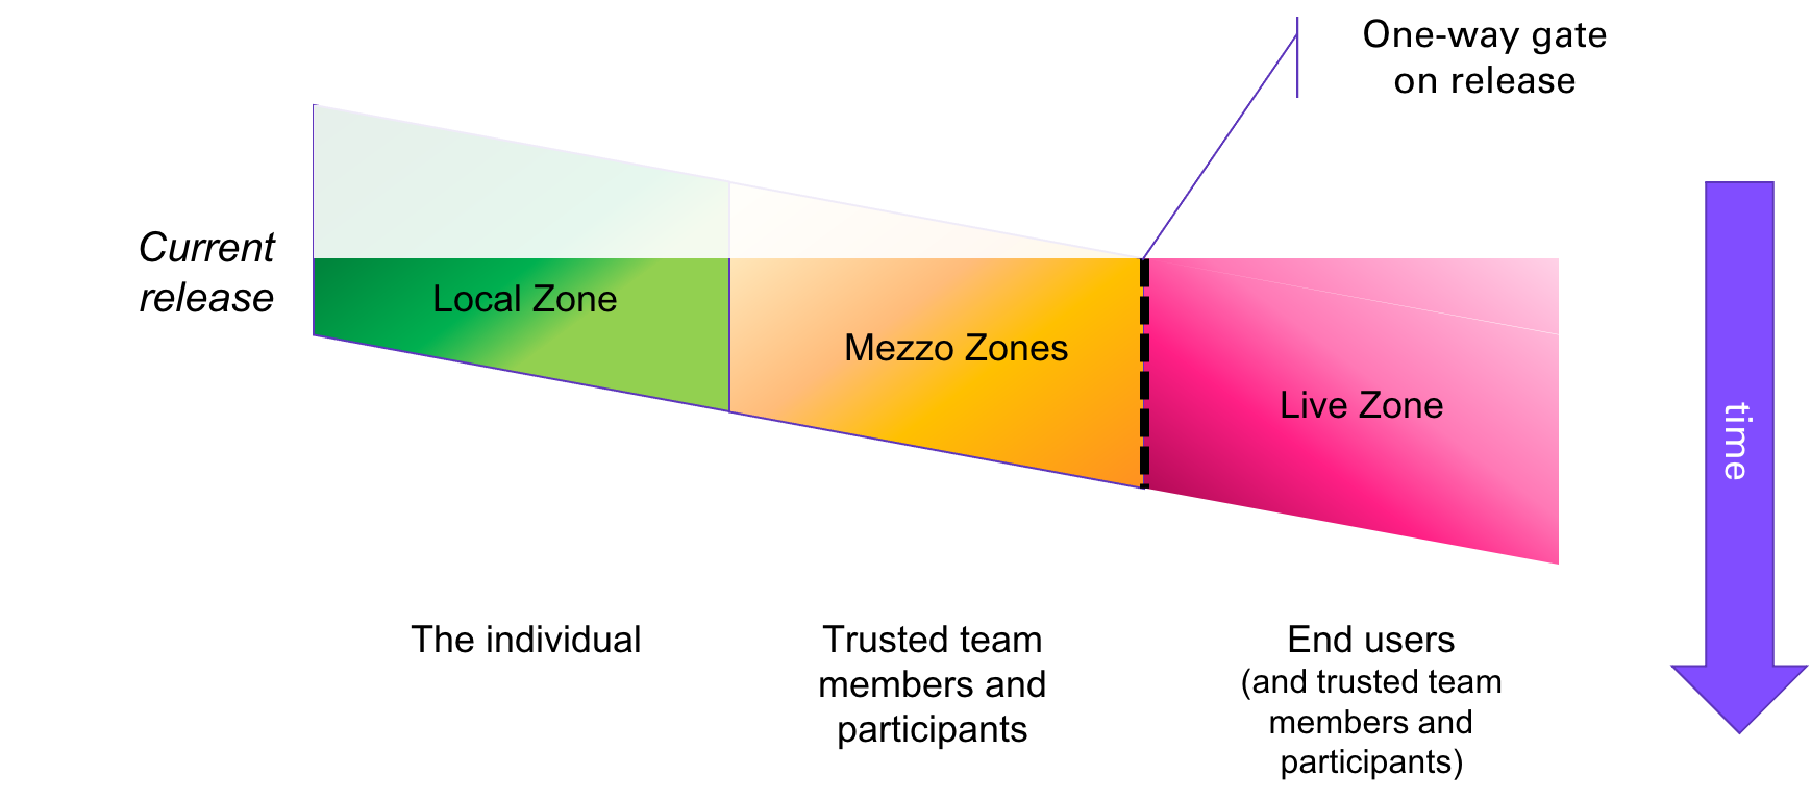
\includegraphics[width=\linewidth]{images/my/control-find-fix-zones-a.pdf}
    \caption{Control find-fix zones}
    \label{fig:my:control-find-fix-zones-overview}
\end{figure*}

Given the constraints that are faced by the vast majority of mobile app developers, of rollouts taking many days and of needing to cope with sometimes lengthy delays in app approvals. 

Mention poor behaviour and their effects on app approvals.

TODO Discuss limits on releasing often that lead to an adapted set of working practices, release frequencies, etc. Perhaps do so elsewhere in this thesis?


\section{Mobile Analytics Usage Lifecycle}~\label{section-mobile-analytics-usage-lifecycle}
For projects that incorporate and use Mobile Analytics, it also has a usage lifecycle. It's important to recognise where the outputs come from, and then how they are interpreted, applied, actioned, and where and how the evidence can be obtained of the effects of applying results of the mobile analytics outputs.

\begin{figure*}
    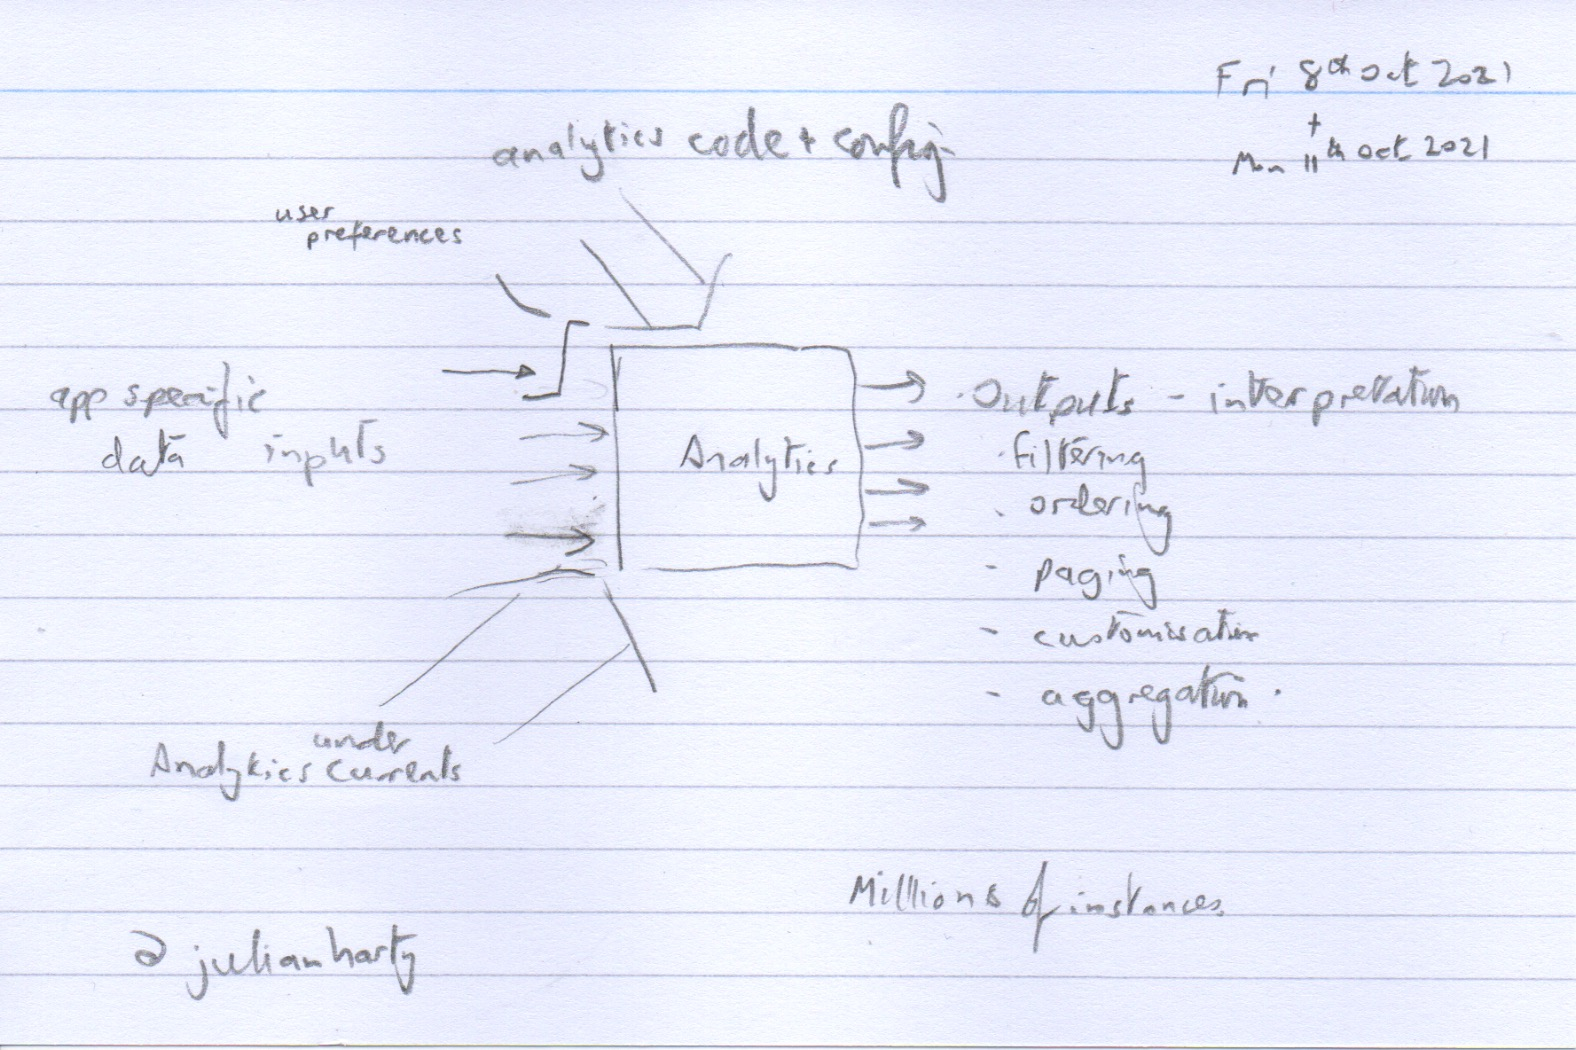
\includegraphics[width=\linewidth]{images/rough-sketches/outputs_from_inputs_code_config-11-oct-2021.jpeg}
    \caption{Outputs from Inputs, Code, and Config (draft)}
    \label{fig:outputs_from_inputs_code_config}
\end{figure*}

Figures \ref{fig:outputs_from_inputs_code_config} and \ref{fig:analytics-feedback-cycle} are connected and illustrate firstly what may affect the outputs pertaining to mobile analytics in isolation, and then how the contents of the first figure fit into a larger, holistic feedback cycle. 

\begin{figure*}
    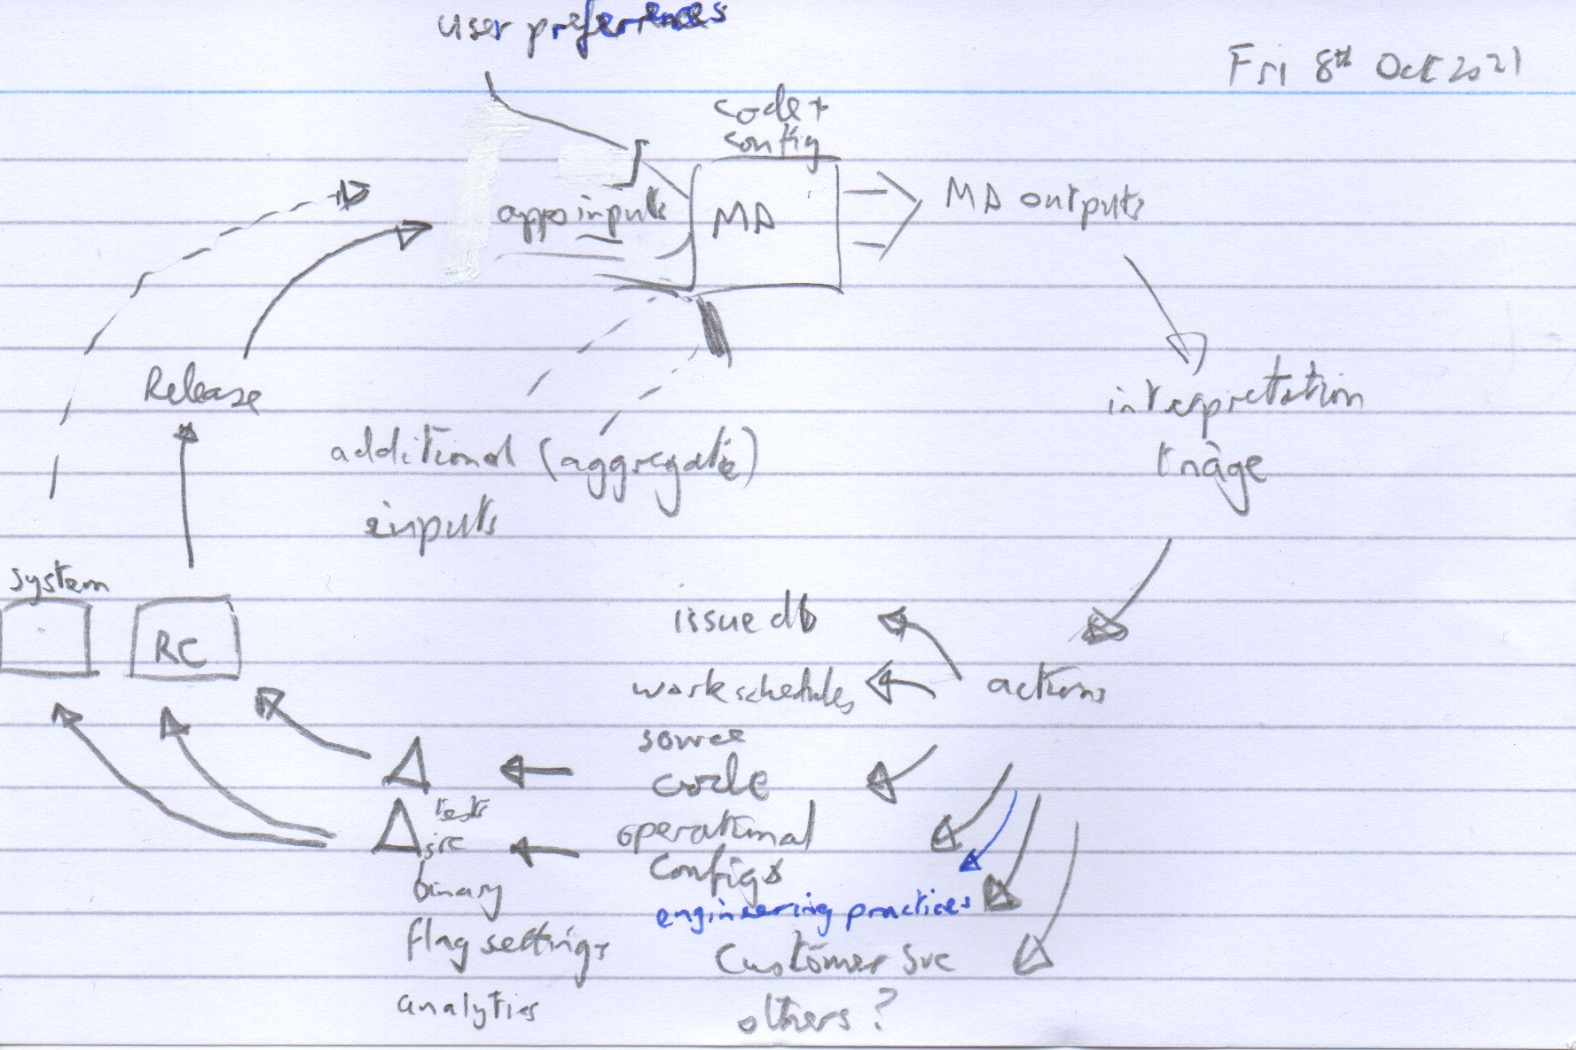
\includegraphics[width=\linewidth]{images/rough-sketches/analytics-feedback-cycle-11-oct-2021.jpeg}
    \caption{Analytics Feedback cycle (draft)}
    \label{fig:analytics-feedback-cycle}
\end{figure*}

In the first of the figures, \ref{fig:outputs_from_inputs_code_config}, working from right to left there is the interpretation of the outputs of a mobile analytics service~\sidenote{The service is provided to developer. It includes the code and configuration that are instantiated to provide analytics processing and reporting aspects; it excludes software running on the mobile devices.}. The interpretation is influenced by the various outputs and how they are used by whoever performs the interpretation. The analytics outputs are influenced by four elements: 
\begin{enumerate}
    \itemsep0em
    \item The service, which includes the instantiation of the server side code and configuration; 
    \item The app-specific inputs (such as failure data e.g. stack traces); 
    \item User-oriented preferences, settings, and so on (e.g. whether analytics reporting is enabled or blocked); and 
    \item Analytics undercurrents (the underlying data and sources may be unavailable to the developers however it may be used by the analytics service, for instance to provide peer-group reports).
\end{enumerate}

The figure illustrates the system for one app, however the analytics service may have as many as millions of instances e.g. Google Play provides one instance of the Google Play Console dashboard for each Android app live in the Play Store. \emph{The instances are unlikely to be identical; they may differ in the analytics code and configuration for instance if Google is running A/B experiments for Google Play Console or performing phased rollouts of new features and/or releases.} Developers may also have customised their analytics service, so they may have distinct views, reports, and interpretations than their co-developers and other colleagues.

In summary, the interpretation of what a mobile analytics service provides depends on the outputs which may, in turn, be affected by their navigation and use. 

The outputs are driven through a combination of elements; these are mainly outside the direct control of the developer, however the developer may be able to influence them. Examples of how the developer may be able to influence these include:
\begin{itemize}
    \itemsep0em
    \item Analytics code and configuration: the developer may be able to opt-in to early experience programs (EEP's), \emph{etc.} These may include new features, reports, and so on that are not available to developers who are not part of these EEP's.
    \item User preferences: the app may include facilities and/or guides aimed at encouraging the user to opt-in (or out) of providing analytics data.
    \item App-specific data inputs - here are some representative examples: the developer may be able to add additional calls to a suitable Mobile Analytics API, or to generate logging messages that are interpreted as failures by the mobile analytics client-side processing. Some Mobile Analytics APIs also provide programmatic access to discard analytics events at run time.  
    \item Analytics undercurrents: the developer may be able to select the peer applications and/or peer category their app is compared with.
\end{itemize}

As mentioned earlier, \secref{fig:analytics-feedback-cycle} subsumes \secref{fig:outputs_from_inputs_code_config} in the upper, central and right areas. Interpretation of the mobile analytics outputs is the first stage in being able to act on them. Triage is the next, and for those deemed sufficiently pertinent are likely to lead to actions. These actions may play out in one or more theatres, for instance in an issues database, in work schedules, in source code, operational configurations, and/or in engineering practices. They may also lead to actions in customer service, and others (such as user-oriented material \emph{e.g.} in online FAQs).

The actions may also result in changes to the sources for the mobile apps and/or in systems that support the app. Changes in the mobile app may form part of a Release Candidate (RC in the diagram) and subsequently in a release. If the release is deployed and then used it will provide fresh app-specific data inputs, and these then feed the mobile analytics.

\begin{figure*}
\RawFloats
\centering
\begin{minipage}{.70\textwidth}
  \centering
  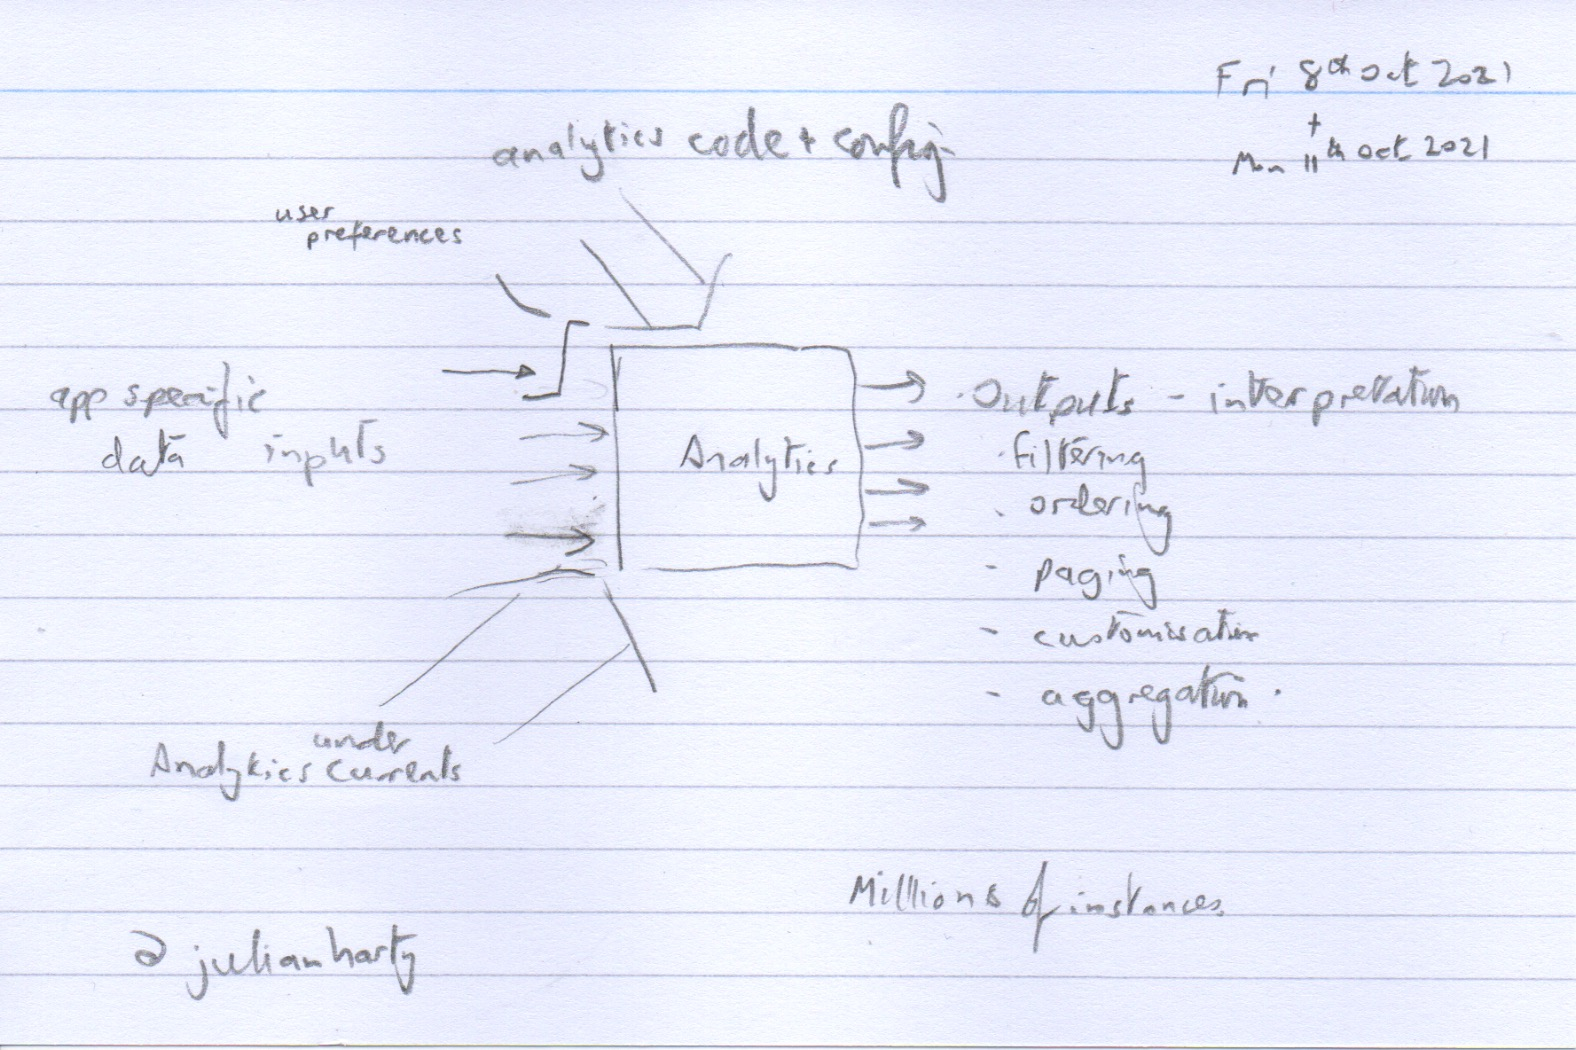
\includegraphics[width=\linewidth]{images/rough-sketches/outputs_from_inputs_code_config-11-oct-2021.jpeg}
  \captionof*{figure}{Outputs from Inputs, Code, and Config (draft)}
\end{minipage}\hfill%
\begin{minipage}{.70\textwidth}
  \centering
  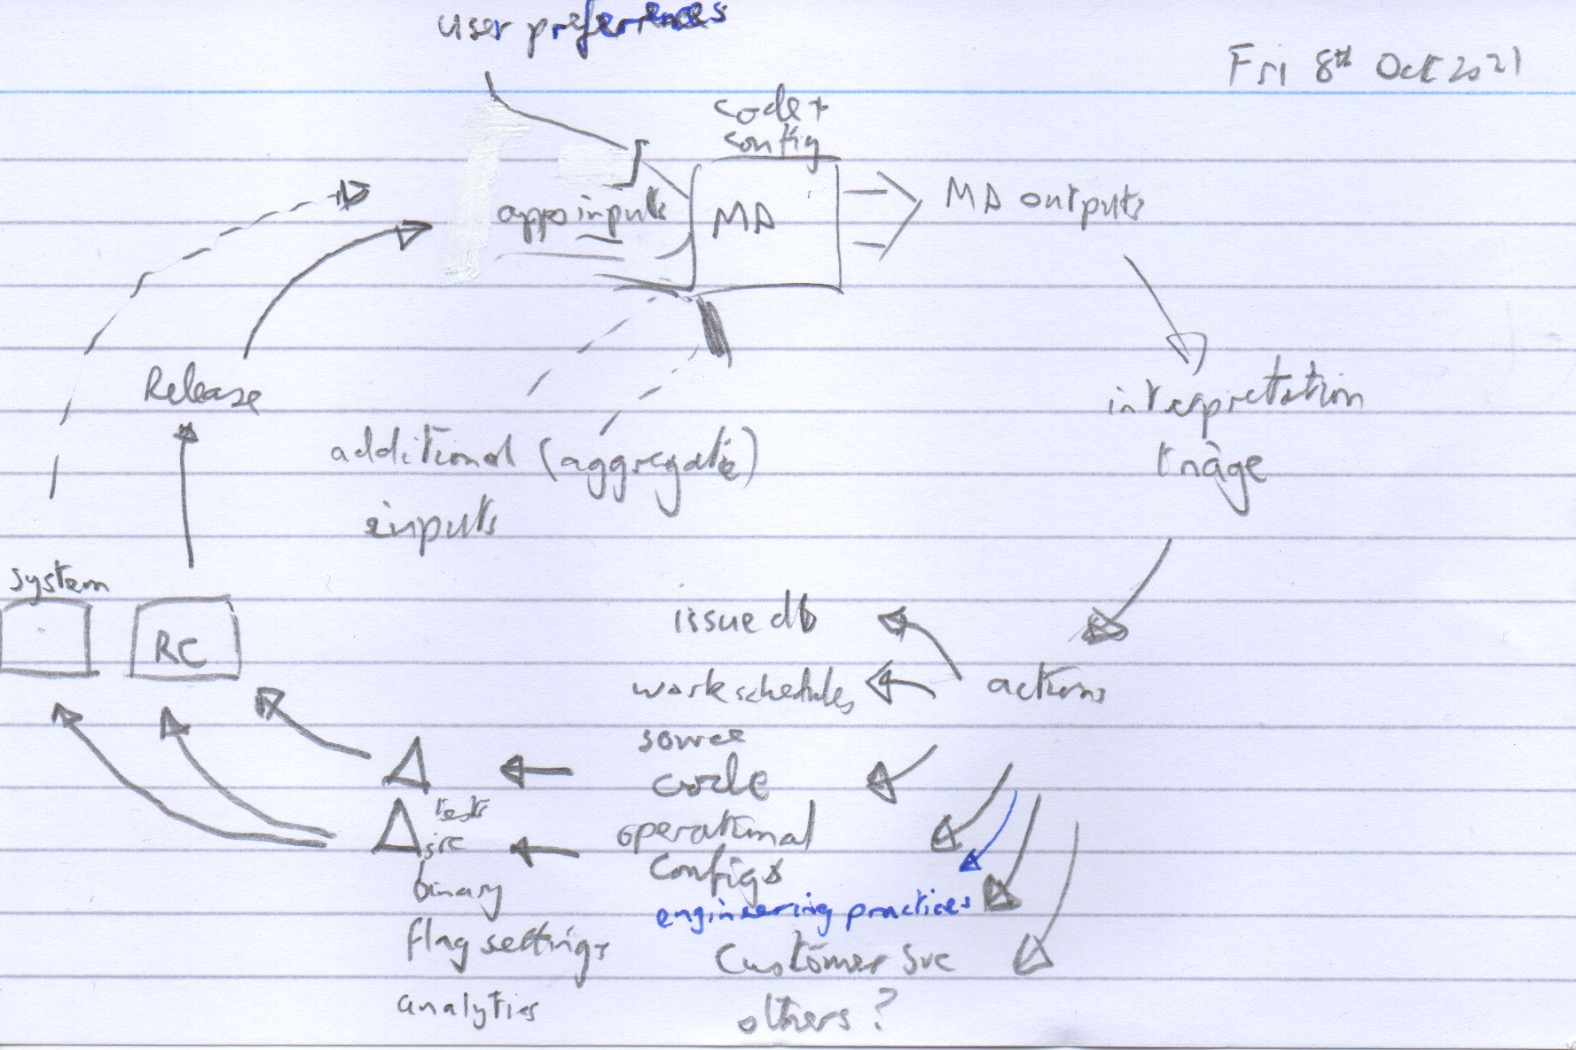
\includegraphics[width=\linewidth]{images/rough-sketches/analytics-feedback-cycle-11-oct-2021.jpeg}
  \captionof*{figure}{Analytics Feedback cycle (draft)}
\end{minipage}
    \caption{Mobile Analytics Contexts}
    \label{fig:mobile-analytics-contexts}
\end{figure*}


FYI: Figure ~\ref{fig:mobile-analytics-contexts} incorporates \secref{fig:outputs_from_inputs_code_config} and \secref{fig:analytics-feedback-cycle} and keeps the two figures together in the document. I've yet to work out if it'll work well with the text, it's here as a reminder I want to improve the links between these two related drawings.



\section{Information sources for app developers}
Developers want and need to know how well their apps are performing from various perspectives such as: growth and adoption (\emph{``do we have more users and are they using the app [more] often?"}), users' ratings and reviews (\emph{``do they like our work?"} and in terms of quality (\emph{``does it perform well? is it fast and reliable?"}). 

\begin{figure*}
    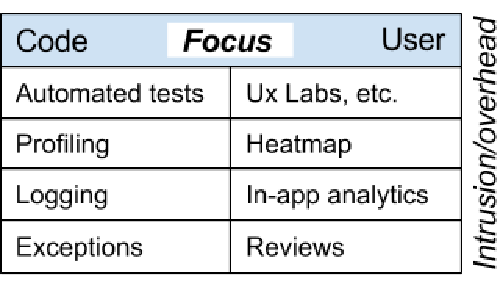
\includegraphics[width=\linewidth]{images/ComparingTechniquesRHS.pdf}
    \caption{Comparing Techniques}
    \label{fig:comparing_techniques}
\end{figure*}

\begin{table}
\RawFloats
    \parbox{.40\linewidth}{
        \centering
        \small
        \begin{tabular}{lll}
            Technique  & Gen. Effort & Usage Effort  \\
            \hline
            Automated Tests  & High  & Medium \\ 
            Profiling   & 1 & 1 \\
            Code Quality tools & 1 & 1 \\
            Logging   & 1 & 1 \\ 
            Exceptions  & 1 & 1 \\ 

        \end{tabular}
        \caption{Focus: Code \label{HRVtable}}
    }
    \hfill
    \parbox{.40\linewidth}{
        \centering
        \small
        \begin{tabular}{ll}
            Technique & vector$_1$  \\
            \hline
            UX labs, etc. & 1  \\ 
            Heatmap & 1  \\ 
            In-app feedback & 1  \\ 
            App-store reviews & 1  \\
        \end{tabular}
        \caption{Focus: User \label{BACtable}}}
    \caption{Comparing techniques}
\end{table}

HRV data in Table \ref{HRVtable} and BAC data in Table \ref{BACtable}.

There are various techniques that can be used to assess aspects of quality of mobile apps. Figure \ref{fig:comparing_techniques} provides a visual overview of eight techniques. Of these four are code-oriented and the remaining four more user- or usage- oriented. They are ordered in approximate rank of the overhead, effort, or intrusion involved of each technique. % MUST-DO continue and expand this argument. Discuss why exceptions were chosen as one of the core elements of this research and PhD thesis.

Google's Google Play app store provides developers with answers to all these niggling questions through a developer-oriented user interface called Google Play Console. 
In Google Play Console they provide various tools, reports and data all aimed at informing developers about how their apps are 'doing' and performing. Broadly, these include an overview page with one line of pre-selected data per app managed by the Google Play \textit{Developer Account}. Then, per app, Google provides an overview dashboard of graphs which, in turn, link to more detailed reports and information which provide greater depth. (Examples are provided in the~\href{appendix-analytics-tools}{\emph{\nameref{appendix-analytics-tools}}} appendix.)  Some graphs only appear when Google's algorithms decide they are relevant, these seem to be related to events and/or volumes of underlying data.




\section{Passive, tacit, and explicit analytics choices}
Various degrees of choices are available depending on how actively the development team wishes to incorporate analytics into their development practices. These include using what already exists, where the data is gathered by others and made available to the developers, here these sources are called \emph{passive analytics}. Developers can choose to take more authority in the data collection, for instance by deciding what data they would like to collect and how they wish to collect it. They can use these tools at various depths, ranging from superficial use to actively maximising the efficacy of using analytics to provide them with the data they believe they need to achieve their outcomes. There is an interesting discussion in a blog article~\sidecite{mukherjee_implicit_versus_explicit_event_tracking_hits_and_misses} on what they term \emph{implicit, or codeless} and \emph{explicit or code-based} event tracking using web analytics tools. The article compares the benefits (hits) and flaws (misses) of both approaches. It also provides a flow chart to help teams select analytics tools that suit their context.

% More reading
% https://web.archive.org/web/20120401053907/http://www.wiikno.com/blog/explicit-vs-implicit-data
% MUST-DO check Patrick's recording of this webinar: https://snowplowanalytics.com/events/explicit-vs-implicit-tracking/ and write up germane items here.


\subsection{Passive Analytics}~\label{subsection-passive-analytics}
Passive analytics are those not actively under the control or influence of the development team, they are provided from other sources such as the operating system or the app store. In the context of this research the passive analytics are all managed by the app store, Google Play, and made available to developers through Google Play Console. As Google states in a US patent,~\emph{``several services provide passive analytics collection such as receiving information about the device type, time of usage, location usage, feature usage, and event reporting."}~\sidecite{googlepatent_hyman2016_collecting_application_usage_analytics}.  

% COULD-DO compare with the concept of passive monitoring https://en.wikipedia.org/wiki/Passive_monitoring however the Wikipedia article doesn't currently add enough to justify citing it or comparing with it.

\subsection{Tacit Analytics}~\label{subsection-tacit-analytics}
Tacit is variously defined as \emph{``Something tacit is implied or understood without question."}~\sidenote{\url{https://www.vocabulary.com/dictionary/tacit}}, \emph{``Understood or implied without being stated."}~\sidenote{\url{https://www.lexico.com/en/definition/tacit}, Note: Lexico.com is a new collaboration between Dictionary.com and Oxford University Press~\url{https://www.lexico.com/about}}, silent, wordless, or noiseless. 
%
It may be something that is inherent in the nature of using many of the third-party analytics libraries. In this research~\emph{tacit analytics} is where developers accept whatever default data is collected by an analytics library without the developer needing to do anything more than integrate the library into their app. 

\subsection{Explicit Analytics}~\label{subsection-explicit-analytics}
Explicit analytics is where developers have actively added code to interact with analytics libraries, for instance by calling methods in the API(s) provided by the library's. There are various degrees of use of the APIs and developers may have various intentions for calling these APIs.

\section{Drilling down into analytics}\label{section-drilling-down-into-analytics}
At the highest level of information, an item and an associated number provides some information: a total crash rate of 99.1 \%, 97K total installs, 37 reviews, and so on. These values may change over time, however if we do not keep track of previous values they cannot be compared, and also relevant information may be hidden behind the totals. The total sums up as many values as exist (from zero values onwards). Some of the reported analytics are of this high-level form.

Totals for subsets of the overall volume of data helps provide additional and potentially relevant information. Relevant subsets for mobile analytics include: date ranges, app releases, platform versions, and many others. Other examples, found in some analytics tools include crash clusters - collections of crash reports considered to be sufficiently similar to enable various individual crashes to be grouped and aggregated. The ability to segment and report on segments allows more detailed analysis than simply observing subsets. 

Comparisons with one or more peer groups provide relational analytics, helping answer: ``how is this app performing compared to various peer groups?" Unless the team has direct access to the data for their peer group, the statistics for the peer group need to be available to a trusted party who perform the comparisons. Some data is publicly available for instance the overall rating of an app together with a limited number of recent reviews and the total installs \textbf{MUST-DO} write up research that uses these sources in the related works chapter, add some of the citations here. There are also commercial services available, and some analytics tools, including Google Play Console, provide these comparisons as part of their services.

Individual records provide the most detail that's available. Note: Developers may be able to create new records and enhance existing records and/or add additional forms of analytics if they want/need more detail. Examples of individual records include stack traces for crashes and similar internal state data for ANRs. Some analytics tools allow developers to capture and subsequently see individual records, for instance details of an item added to an e-commerce shopping cart by an end user. Mobile analytics ultimately can only report on data that is provided to it. 

The analytics tool may or may not make aspects of the data available to the users of the tool. As a concrete example, Google Play Console provides developers access to individual reviews (with their associated rating), it also used to provide access to crashes and ANRs for several years before removing these and replacing them with summary data in 2018 \textbf{MUST-DO} add reference and cite it.

\textbf{MUST-DO} provide screenshots of category peer groups and custom peer groups. Discuss either here, or in a later chapter, Google's cap on the number of changes to the custom peer group.

Two key points in summary: being able to keep track of analytics as they change over time allows comparisons and trends to be determined. Additional detail can help identify meaningful differences for instance that a crash rate is much higher than the mean for a particular model of smartphone. 

How much information is needed to be actionable? (Thought: This may be more of a research question...)


\textbf{MUST-DO} introduce my concept of resolution.

\textbf{PERHAPS} introduce the concept of app peer groups here?

\begin{figure*}
    \copyrightbox[r]{
        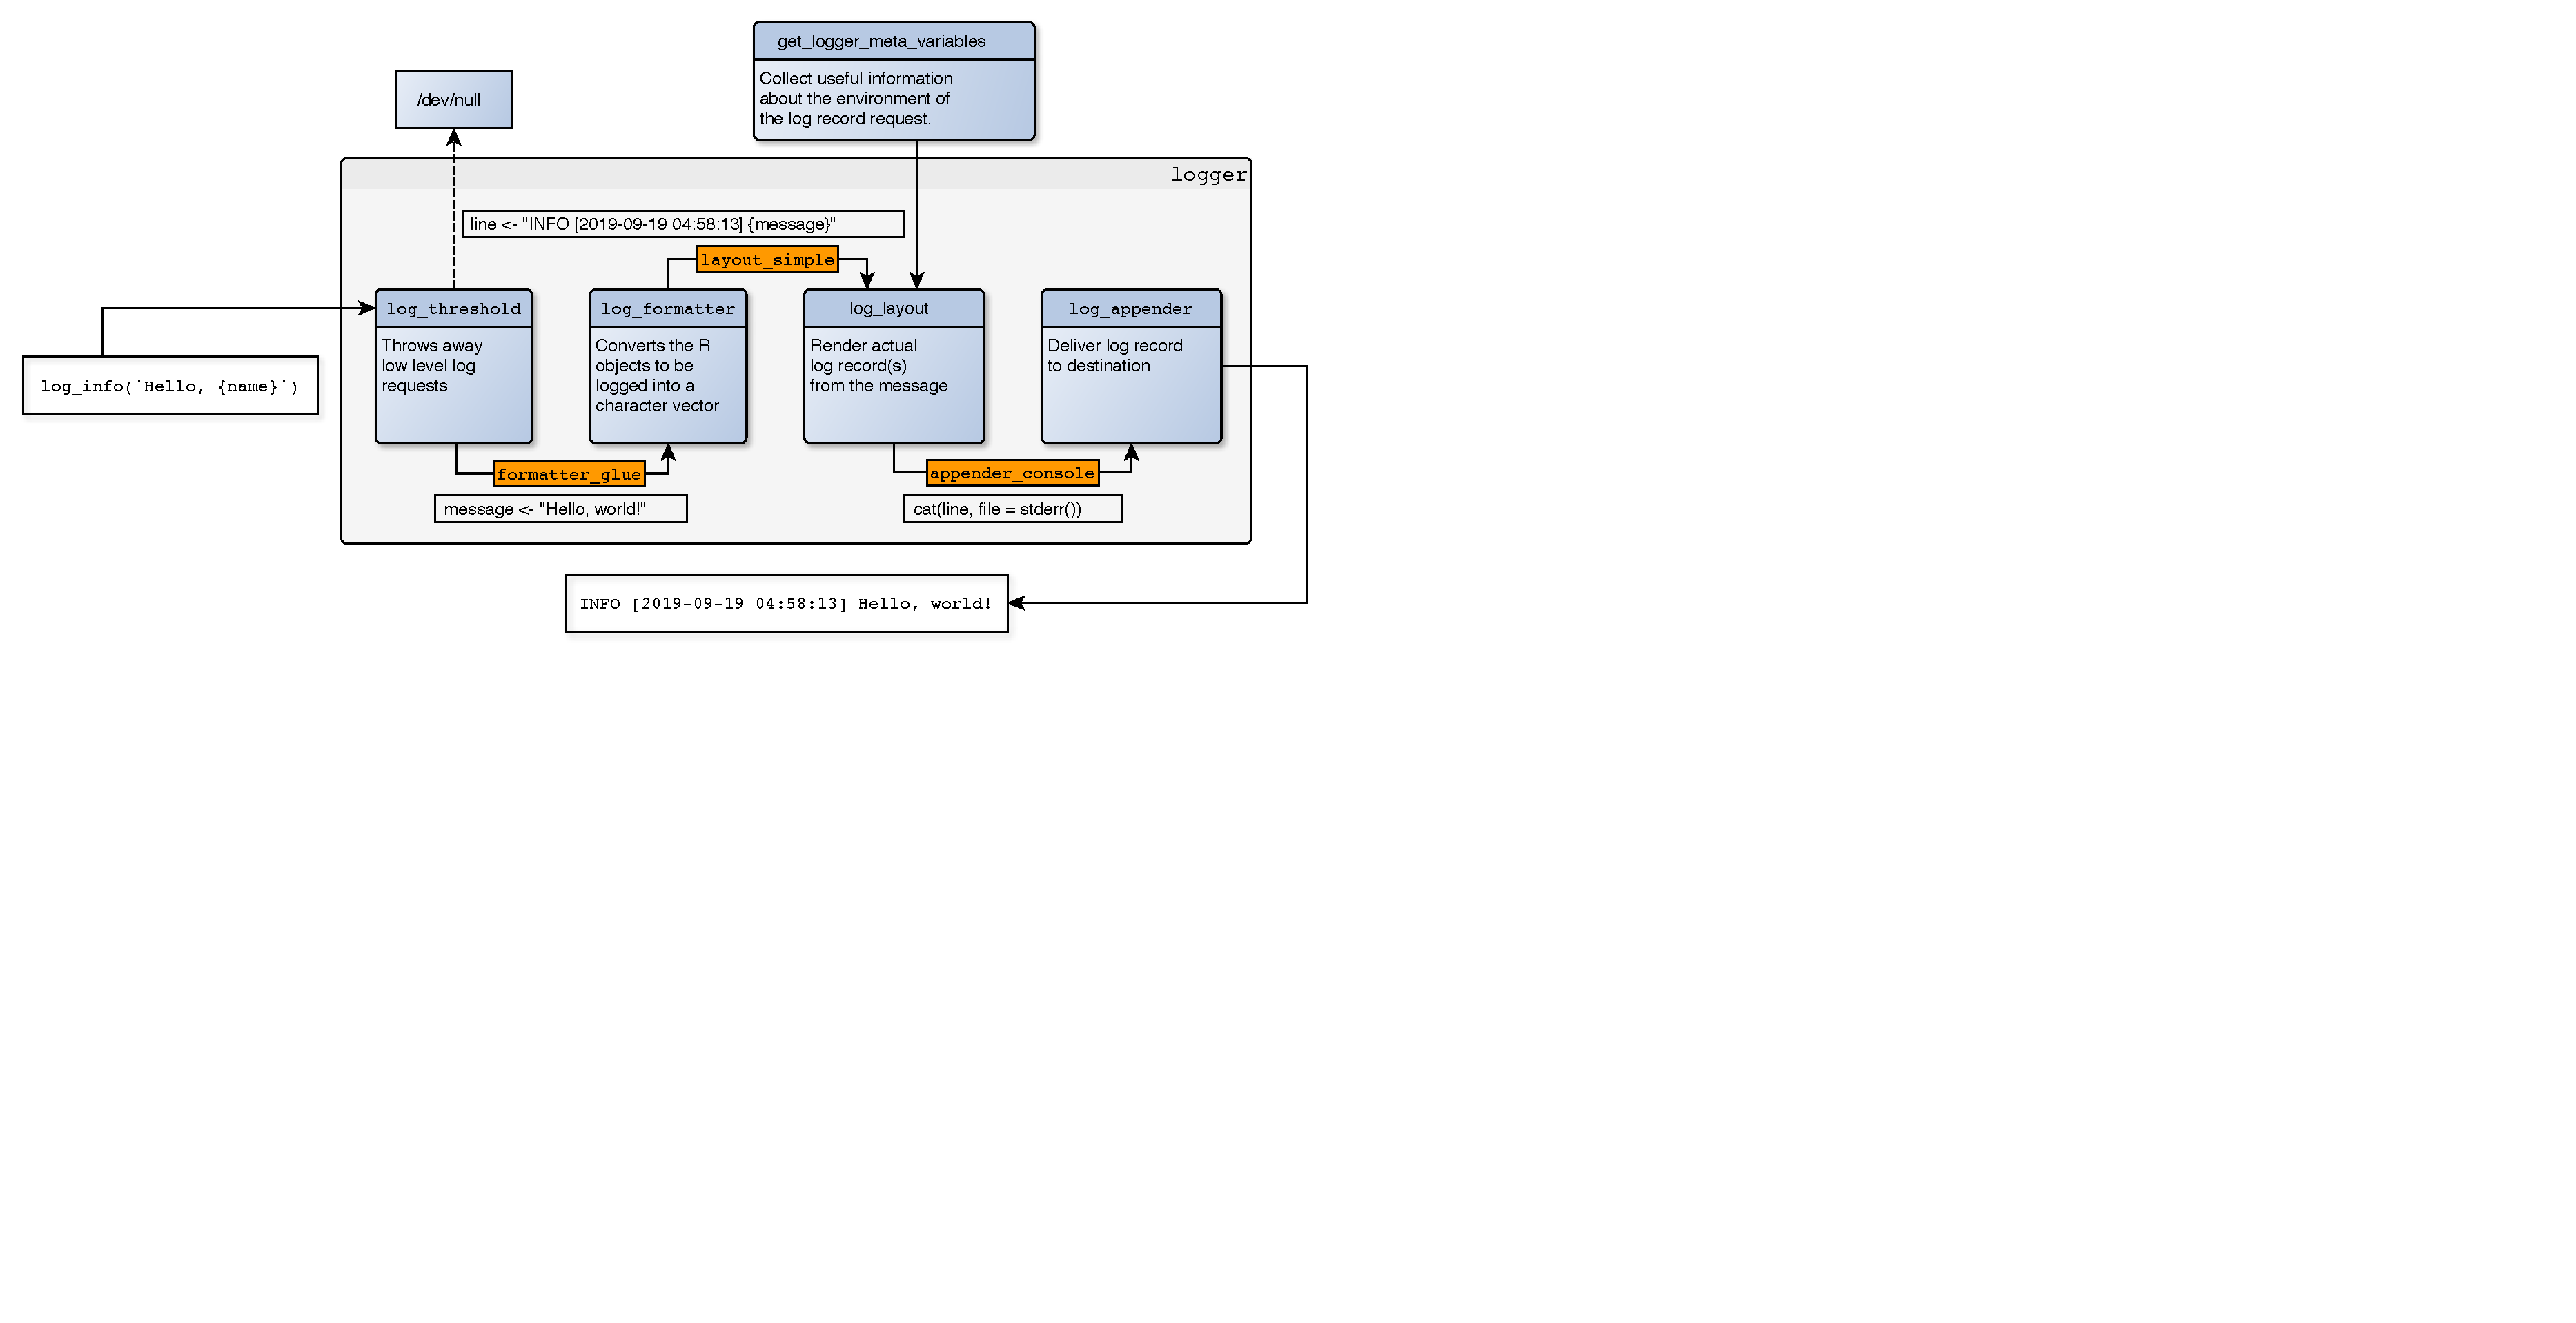
\includegraphics[width=\linewidth]{images/github/loggerstructure.pdf}}
    {\textcopyright \href{{https://twitter.com/daroczig}}{daroczig}\\source: \href{https://github.com/daroczig/logger/blob/master/vignettes/logger_structure.svg}{logger\_structure.svg}}
    \caption{TEMP - to be replaced: Logger Structure from an R Logger project - TBC whether to provide something similar}
    \label{fig:temp_logger_structure}
\end{figure*}

\textbf{SHOULD-DO}, it'd be great to have a figure similar to \url{https://github.com/daroczig/logger/blob/master/vignettes/logger_structure.svg} for platform-level analytics. Temporarily it's included here in Figure~\ref{fig:temp_logger_structure}.



\begin{figure}
    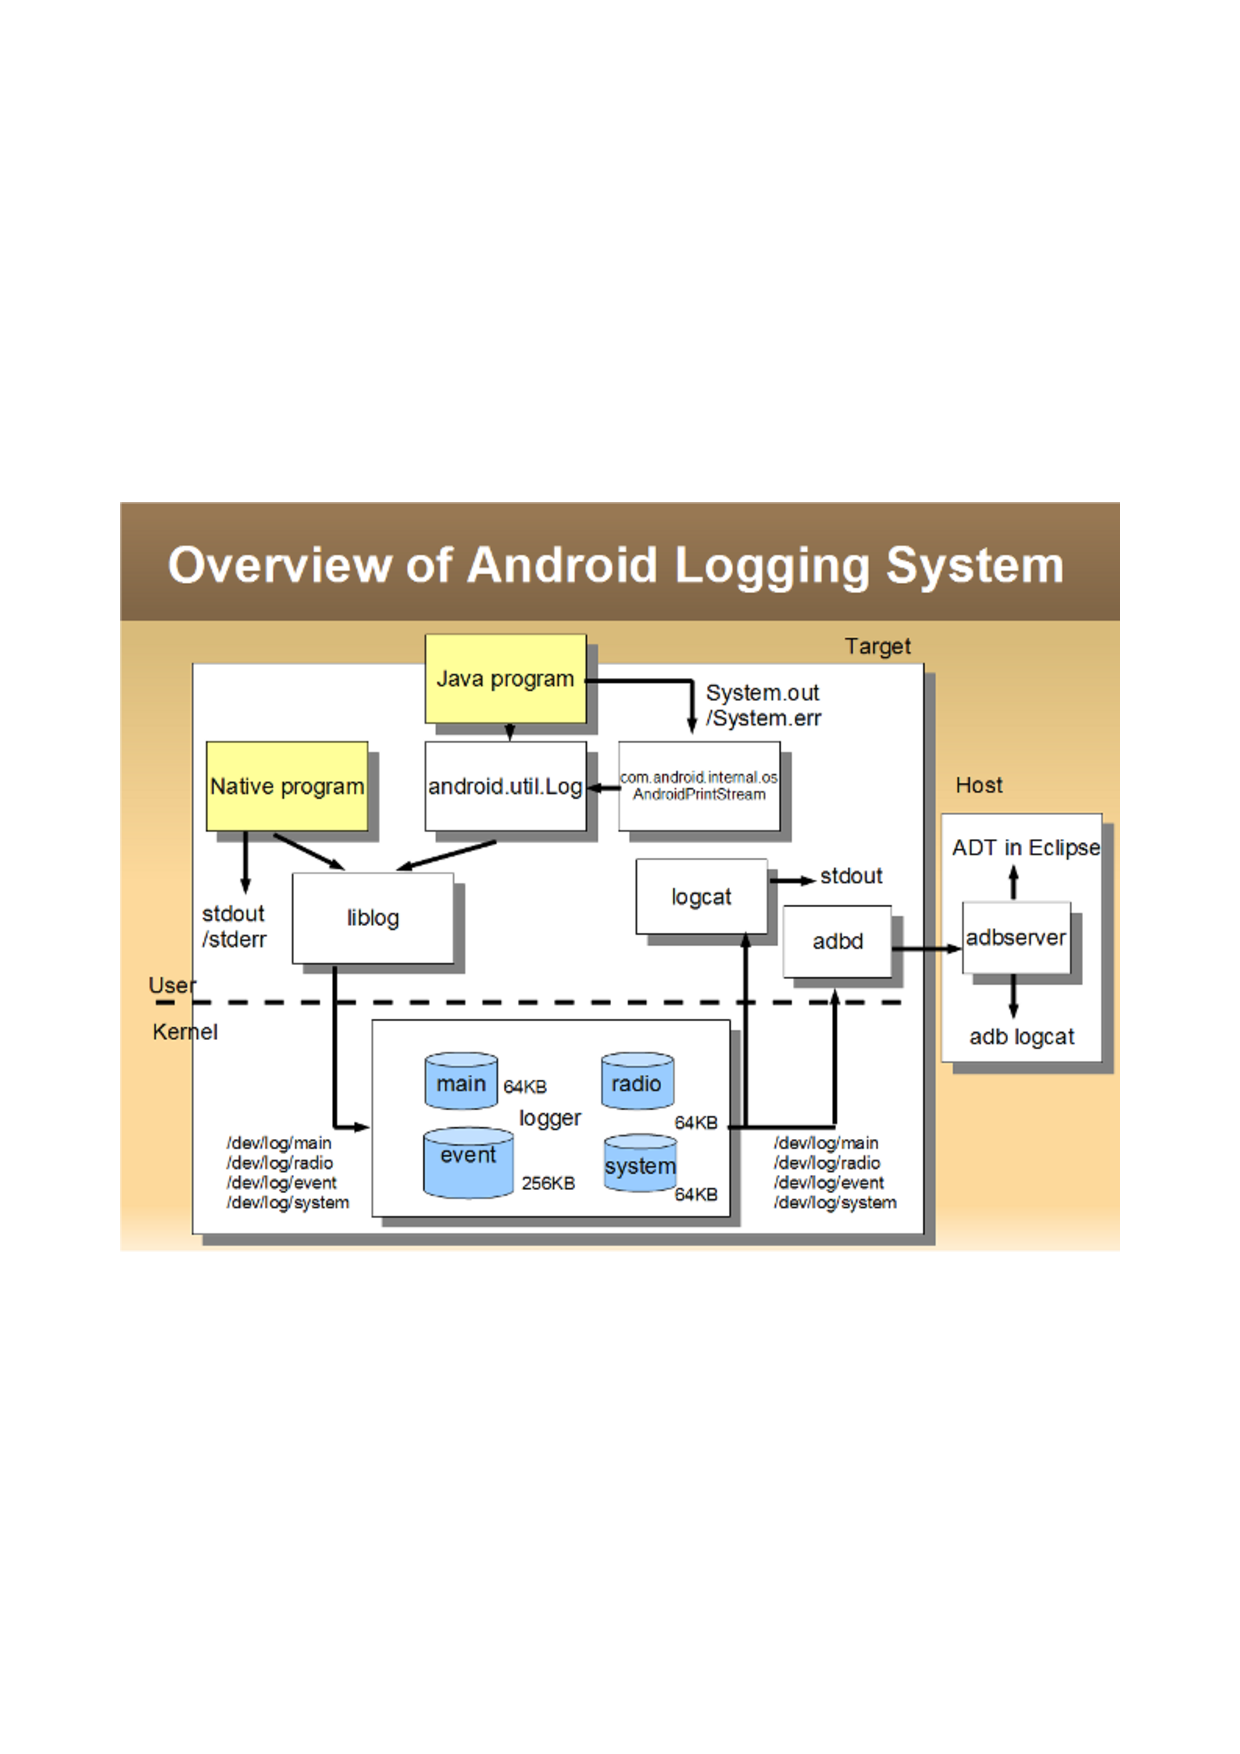
\includegraphics[width=\linewidth]{images/elinux.org/Android-logging-kmc-kobayashi.pdf}
    \caption[Android Logging]{Android Logging\\Source \href{https://elinux.org/Android_Logging_System}{elinux.org/Android\_Logging\_System}, license \href{https://creativecommons.org/licenses/by-sa/3.0/}{creativecommons.org/licenses/by-sa/3.0/}}
    \label{fig:android_logging_circa_2010}
\end{figure}

Figure \ref{fig:android_logging_circa_2010}~\sidenote{Published originally around 2010, see \href{http://blog.kmckk.com/archives/2936958.html}{blog.kmckk.com/archives/2936958.html} (in Japanese).} 
provides a historical perspective of Android logging infrastructure at the time. It appears to predate the additional log used to record crashes \texttt{LOG\_ID\_CRASH}.

Figure~\ref{fig:sources-of-info-with-app-store-background-ch} illustrates various sources of information for apps available in an app store. The sources and communications paths will be considered next. 
% SHOULD-DO Perhaps a Venn diagram would also complement this illustration?

\begin{figure*}
    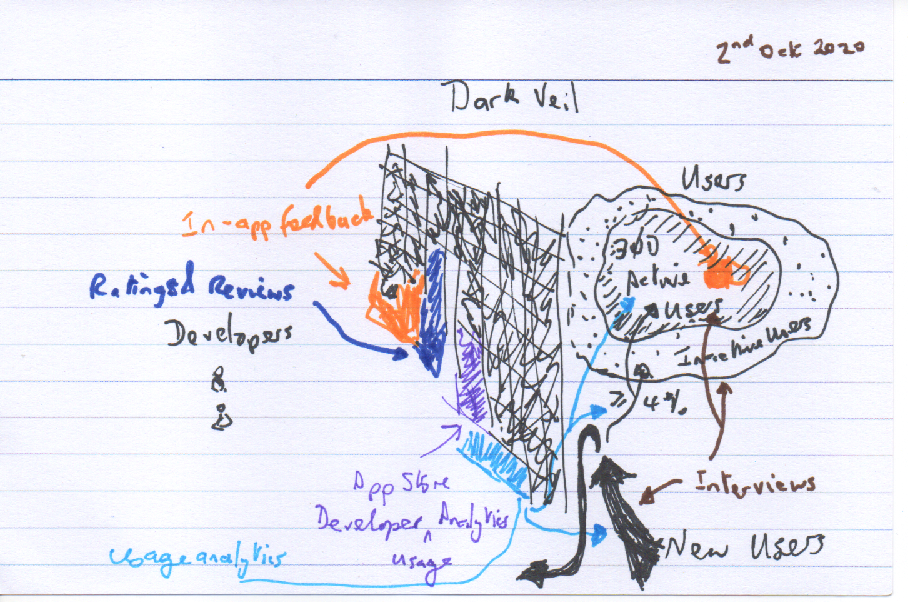
\includegraphics[width=\linewidth]{images/rough-sketches/sources-of-information-with-app-store-1.pdf}
    \caption{Sources of information with an App Store}
    \label{fig:sources-of-info-with-app-store-background-ch}
\end{figure*}

\begin{figure*}
    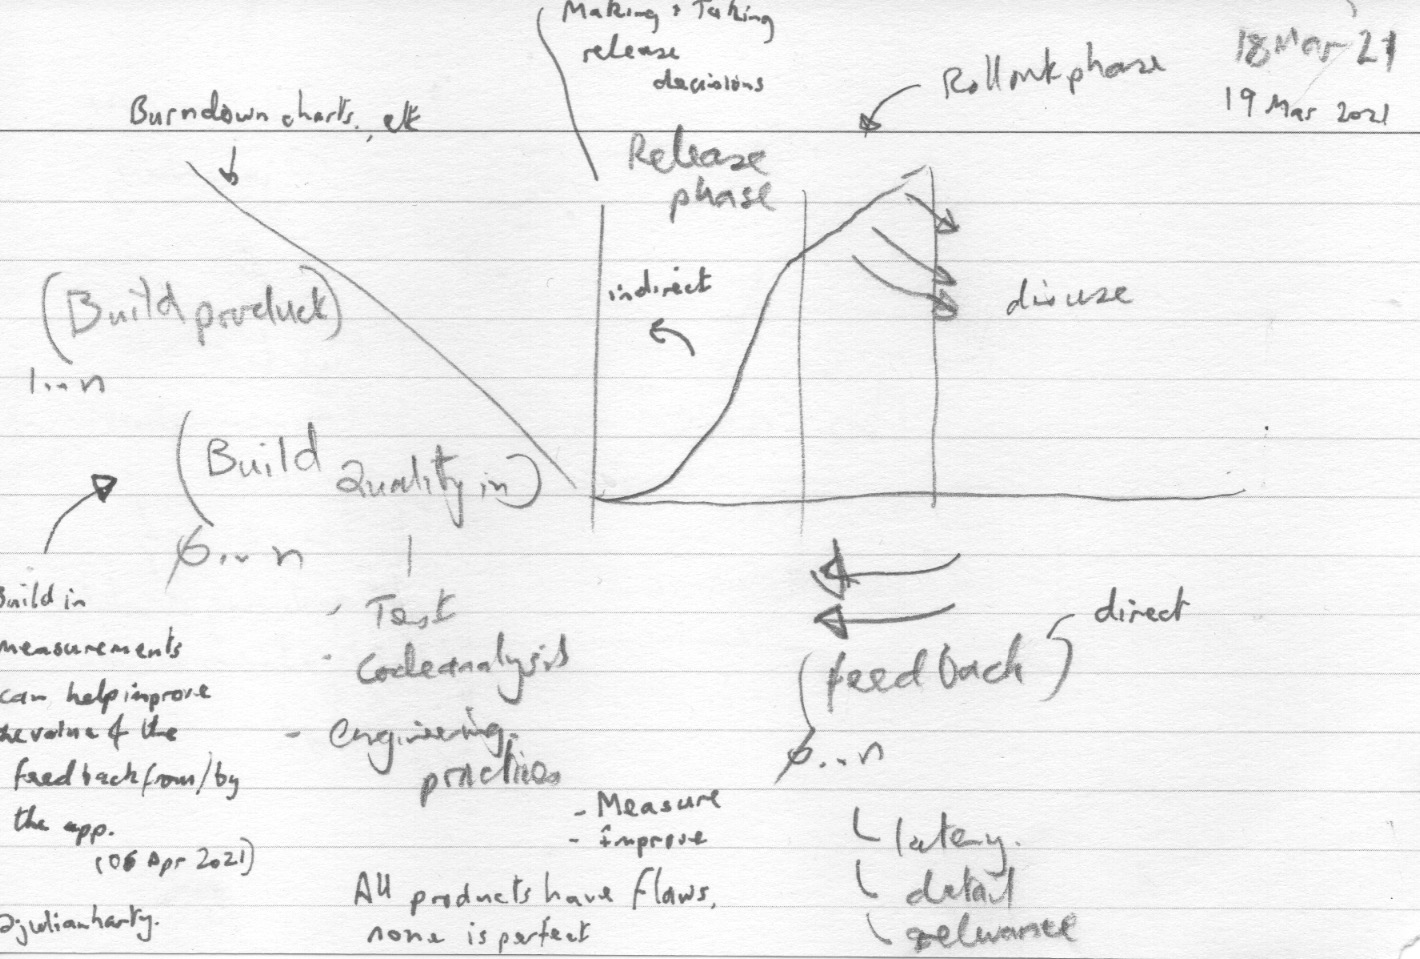
\includegraphics[width=\linewidth]{images/rough-sketches/Red-Thread-Rough-Sketch.jpeg}
    \caption{The lifecycle of a release and where mobile analytics provides feedback}
    \label{fig:red-thread-for-this-thesis}
\end{figure*}

\begin{comment}
\begin{figure*}
    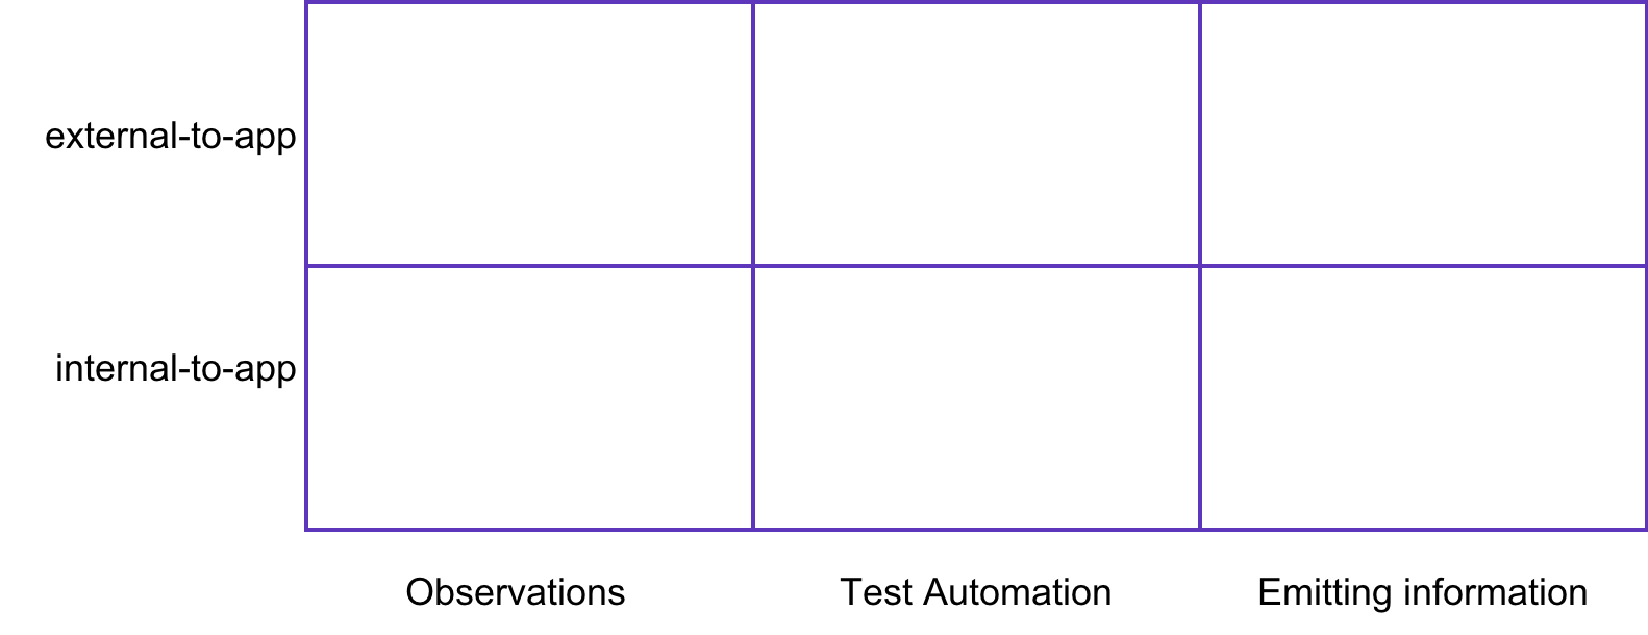
\includegraphics[width=\linewidth]{images/internal-external-table.pdf}
    \caption{Internal and external perspectives of an app}
    \label{fig:internal-external-table}
\end{figure*}
\end{comment}


%\textbf{SHOULD-DO} Expand the following: What is test automation? discuss how mobile apps are tested, the unique aspects of using accessibility interfaces, etc.

